\documentclass[a4paper, 11pt]{article} % Documentklasse und Papierformat festlegen

\usepackage[left=2.5cm, right=2.5cm]{geometry} % Ränder festlegen
\usepackage{fancyhdr} % Um Kopf- und Fußzeilen zu gestalten
\usepackage[utf8]{inputenc} % Encoding für Umlaute
\usepackage[T1]{fontenc} % Font Encoding für korrekte Darstellung von Sonderzeichen
\usepackage[ngerman]{babel} % Sprachpaket für deutsche Sprache
\usepackage{lmodern} % Schriftart
\usepackage{amsmath} % Mathematische Symbole und Funktionen
\usepackage{amssymb} % Mathematische Symbole und Funktionen
\usepackage{graphicx} % Einbinden von Grafiken
\usepackage{caption} % Formatierung von Abbildungs- und Tabellenbeschriftungen anpassen
\usepackage{booktabs} % Erstellen von "schöneren" Tabellen
\usepackage{xcolor} % Farben

\setlength{\parindent}{0em} % Verhindert das Einrücken
\graphicspath{{Img/}} % Pfad zu Grafikken für den Compiler
\captionsetup[figure]{justification=raggedright,singlelinecheck=false} % "justification=raggedright" -> Beschriftungen linksbündig ; singlelinecheck=false -> keine automatische Zentrierung

% Neue Befehlsdefinitionen, um das Erstellen des Deckblattes zu erleichtern und einfacher Anpassungen vornehmen zu können.
\newcommand{\Thema}{FPV Drohnen}
\newcommand{\Unterthema}{Herausforderungen für Hard- und Software}
\newcommand{\Autor}{Henrik Sopart}
\newcommand{\Datum}{\today}




\begin{document}

\begin{titlepage}
    \vspace*{2cm}
    \begin{center}
    {\Huge\bfseries\Thema} \\
    \vspace*{0.8cm}
    {\huge\Unterthema}
    \end{center}
    \vspace*{5cm}

    \begin{table}[h]
        \renewcommand{\arraystretch}{1.9}
        \begin{tabular}{p{6cm}p{10cm}}
            {\large\textbf{Vorgelegt durch}}        & {\large\Autor} \\
            {\large\textbf{Matrikelnummer}}         & {\large\Matrikelnummer} \\
            {\large\textbf{Studiengang}}            & {\large\Studiengang} \\
            {\large\textbf{Wohnort}}                & {\large\Wohnort} \\
                                                    &                                   \\
            {\large\textbf{Art der Arbeit}}         & {\large\ArtDerArbeit} \\
                                                    &                                   \\
            {\large\textbf{Abgabedatum}}            & {\large\Abgabedatum} \\
            {\large\textbf{Bearbeitungszeitraum}}   & {\large\Bearbeitungszeitraum} \\
            {\large\textbf{Prüfer}}                 & {\large\Pruefer} \\
        \end{tabular}
        \label{tabelle_deckblatt}
    \end{table}

\end{titlepage}

\tableofcontents
\thispagestyle{empty}
\setcounter{page}{0}


%%% Henrik Sopart, 836188, Latex-Projekt %%%%

\section[A]{B}


%%% Henrik Sopart, 836188, Latex-Projekt %%%%

\section[FPV-Drohnen]{FPV-Drohnen}
    \subsection[Besonderheiten]{Besonderheiten}
        FPV-Drohnen, auch bekannt als Racing- oder Freestyle-Drohnen, besitzen erhebliche Unterschiede
        im Vergleich zu handelsüblichen Drohnen wie beispielsweise der „DJI Mavic 3“. In der folgenden
        Tabelle werden die Unterschiede der beiden Typen gegenübergestellt. Im Anschluss wird genauer
        auf die Unterschiede in der Steuerung und der Komplexität eingegangen.

        \begin{table}[h]
            \renewcommand{\arraystretch}{1.5}
            \begin{tabular}{p{3cm}p{5.86cm}p{5.86cm}}
                \toprule
                \textbf{Merkmal} & \textbf{Handelsüblich} & \textbf{FPV} \\
                \midrule
                Steuerung                       & Unterstützungen durch Assistenzsysteme wie GPS oder Hinderniserkennung und vorprogrammierte Flugmodi\cite{Mavic3DJI}                                                              & Im Normalfall keine Assistenzsysteme oder Flugmodi vorhanden \\
                Sichtverhältnisse               & Flug über Sichtlinie oder Bildschirm, welcher an der Fernsteuerung befestigt ist und das Videosignal empfängt                                                                     & Flug mit einer FPV-Brille, welche das Videosignal empfängt \\
                Verwendungszweck                & Fotografie, Videografie, Vermessungstechnik, Such- und Rettungsarbeiten, Landwirtschaft                                                                                           & Rennen, Wettbewerbe, Freestyle-Flüge, sehr dynamische Videografie \\
                Kamera                          & Meist eine mittels Gimbal stabilisierte Kamera, welche an der Unterseite der Drohne befestigt ist und sich nach oben und unten neigen lässt                                       & Meist zwei in einem festen Winkel montierte Kameras. Eine vorne im Rahmen, die das Bild zur FPV-Brille überträgt. Eine, die auf dem Rahmen befestigt wird und das Video aufnimmt (Actioncam) \\
                Akkulaufzeit                    & Meist deutlich höhere Akkulaufzeiten, beispielsweise bis zu 46 Minuten bei der Mavic 3\cite{Mavic3DJI}                                                                            & Meist deutlich geringere Akkulaufzeit, beispielsweise 5\dq FPV-Drohne 4 bis 10 Minuten, abhängig von der Flugweise \\
                Geschwindigkeit und Agilität    & Geringere Geschwindigkeit und Agilität, die Mavic 3 ist beispielsweise auf \qty{75,6}{\kilo\metre\per\hour} und einem Nickwinkel von maximal 35 Grad beschränkt\cite{Mavic3DJI}   & Hohe Geschwindigkeiten von weit über \qty{150}{\kilo\metre\per\hour} möglich, kein begrenzter Nickwinkel \\
                \bottomrule
            \end{tabular}
            \caption{Unterschiede}
            \label{tabelle_unterschiede}
        \end{table}

    \newpage
    \subsection[Steuerung]{Steuerung}
        Die Steuerung einer FPV-Drohne unterscheidet sich im Wesentlichen in zwei Punkten von der einer
        herkömmlichen. Zum einen bietet die FPV-Drohne im Normalfall keinerlei Assistenzsysteme, zum anderen
        ist die Reaktion der Drohne auf an der Fernsteuerung eingegebene Befehle eine andere. Sobald sich
        bei einer herkömmlichen Drohne beide Sticks der Fernsteuerung in der neutralen Position in der Mitte
        befinden, bleibt die Drohne in der Luft stehen. Wird nun der rechte Stick um das Maximale nach vorne
        bewegt, neigt sich die Drohne nach vorne und beschleunigt. Da die Neigung durch diverse Assistenzsysteme
        begrenzt ist, besteht kein Risiko, dass die Drohne „vorne überkippt“. Wird nun die Fernsteuerung
        losgelassen, bewegt sich der Stick wieder in die neutrale Position und die Drohne bleibt in der Luft
        stehen. Vereinfacht lässt sich sagen, dass die Bewegung am Stick in einen Winkel der Drohne resultiert.
        Die Leistung der Motoren wird automatisch angepasst, um (in diesem Beispiel) den Vorwärtsflug auf
        gleichbleibender Höhe zu ermöglichen. Die Höhe wird über den linken Stick kontrolliert. Allerdings
        geschieht dies relativ zur benötigten Drehzahl, um die Drohne in dieser Höhe zu halten. Befindet sich
        beispielsweise der linke Stick in der neutralen Position, drehen die Propeller so schnell, dass die
        Drohne weder sinkt noch steigt. Wird nun der Stick maximal nach vorne bzw. hinten betätigt, erhöht
        beziehungsweise verringert sich die Drehzahl der Motoren um einige Prozent, damit die Drohne langsam
        steigen beziehungsweise sinken kann. Bei einer herkömmlichen Drohne ist dementsprechend für keine Achse
        eine kontinuierliches Eingreifen durch den Piloten erforderlich. \\
        \\
        Im Vergleich hierzu würde eine FPV-Drohne, bei der der rechte Stick maximal nach vorne gedrückt wird,
        unkontrolliert nach „vorne kippen“ und sich um diese Achse drehen, bis es zum Absturz kommt. Zusätzlich
        gibt es bei FPV-Drohnen keine neutrale Stickposition, bei welcher die Drohne an der Stelle stehen bleibt.
        Jeder Befehl der Fernsteuerung wird ausgeführt. Vereinfacht bedeutet dies, dass eine Bewegung am Stick
        nicht in einem Winkel, sondern in einer Drehgeschwindigkeit um die gesteuerte Achse resultiert. Auch die
        Höhensteuerung funktioniert anders als bei einer herkömmlichen Drohne. Am einfachsten lässt sich dies mit
        einem Potenziometer vergleichen. Befindet sich der linke Stick ganz hinten, drehen die Propeller nicht.
        Wird diese nun nach vorne bewegt, erhöht sich die Drehzahl bis auf den maximalen Wert. Wird die Fernsteuerung
        nun losgelassen, behält die Drohne diese Drehzahl bzw. Drehgeschwindigkeit bei. Da die Bewegung einer Achse
        nur durch direktes Eingreifen des Piloten zu stoppen ist und diese Bewegung nicht wie bei einer herkömmlichen
        Drohne weitere Achsen ansteuert, um beispielsweise einen Vorwärtsflug mit gleichbleibender Höhe zu ermöglichen,
        ist ein kontinuierliches Eingreifen durch den Piloten zwingend erforderlich.

    \subsection[Komplexität]{Komplexität}
        Da die meisten herkömmlichen Drohnen für eine große Zielgruppe entwickelt wurden, sind keine technischen
        Fähigkeiten oder Vorkenntnisse erforderlich, um mit einer solchen Drohne Luftaufnahmen zu erstellen.\cite{shon2022}
        Durch das Zusammenspiel unterschiedlichster Sensoren, wie beispielsweise eine Hinderniserkennung und GPS,
        wird das Risiko für die Drohne minimiert. Zusätzlich erleichtern es Technologien wie Geofencing dem Piloten,
        innerhalb der rechtlichen Grenzen zu fliegen. \\
        \\
        Da FPV-Drohnen immer populärer werden, haben sich in den letzten Jahren neue Möglichkeiten gefunden, in
        dieses Hobby einzusteigen. Seit 2021 bietet die Firma „DJI“ zwei FPV-Drohnen an. Diese müssen nicht selbst
        zusammengebaut werden und erfordern ähnlich wie herkömmliche Drohnen keinerlei technische Fähigkeiten oder
        Vorkenntnisse.\cite{DJIAvatar}\cite{DJIFpv} Da diese Drohnen jedoch proprietäre Komponenten verwenden, auf welche der Käufer keinen Einfluss
        hat, wird auf diese im weiteren Verlauf dieser Arbeit nicht weiter eingegangen. \\
        \\
        Bis vor einigen Jahren gab es nur die Möglichkeit, sämtliche Komponenten wie beispielsweise Motoren,
        Controller, Kamera oder den Rahmen einzeln zu kaufen und sich so seine eigene Drohne zu bauen. Dies
        erfordert ein hohes Maß an technischem Wissen und technischen Fähigkeiten, jedoch erhält man die Möglichkeit,
        die Drohne individuell auf die Bedürfnisse des Piloten anzupassen. Beispielsweise würde für eine Drohne,
        welche Aufnahmen in den Alpen anfertigen soll die Akkulaufzeit eine Priorität sein und aus diesem Grunde
        schwächere, aber effizientere Motoren zum Einsatz kommen. Hingegen würde eine Drohne, welche Autos
        auf einer Rennstrecke verfolgt, leistungsstarke Motoren erhalten. \\
        \\
        In der folgenden Abbildungen werden die oben beschriebenen Unterschiede sichtbar. In Abbildung \ref*{HandelsueblicheDrohne}
        ist eine handelsübliche Drohne zu sehen, in Abbildung \ref*{FpvDrohne} eine FPV-Drohne.

        \vspace{1.2cm}
        \begin{figure}[h]
            \centering
            \begin{subfigure}[b]{0.45\textwidth}
                \centering
                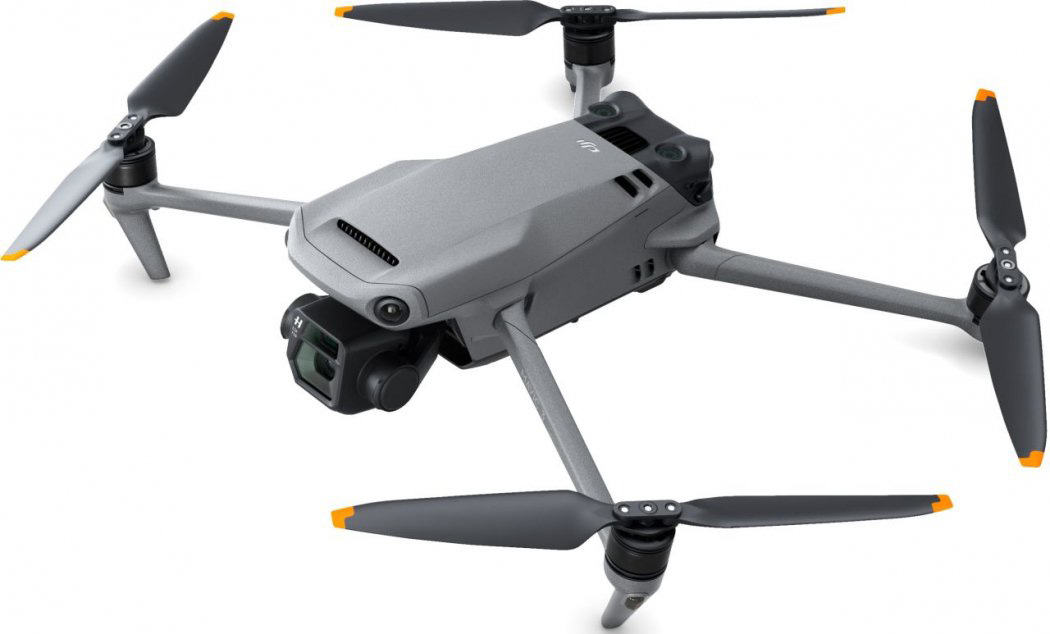
\includegraphics[width=\textwidth]{Img/Bild_DJIMavic3.jpg}
                \caption{Handelsübliche Drohne: DJI Mavic 3\cite{BildMavic3}}
                \label{HandelsueblicheDrohne}
            \end{subfigure}
            \hfill
            \begin{subfigure}[b]{0.45\textwidth}
                \centering
                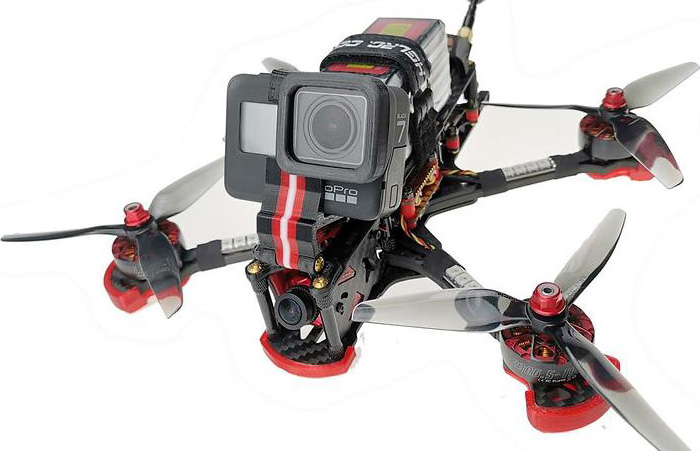
\includegraphics[width=\textwidth]{Img/Bild_FPV.jpg}
                \caption{FPV-Drohne: HGLRC FPV Sector 5 V3\cite{BildFpv}}
                \label{FpvDrohne}
            \end{subfigure}
               \caption{Beispielbilder}
               \label{BeispielBilder}
       \end{figure}
\section[Bauteile]{Bauteile}
    Sowohl FPV-Drohnen als auch normale Drohnen verwenden eine Vielzahl von Bauteilen, um Flüge zu ermöglichen und zu kontrollieren. Dazu gehören beispielsweise Propeller, Akkus, Steuerungen und Sensoren. All diese Bauteile haben die gleichen grundlegenden Funktionen, wie zum Beispiel die Bereitstellung von Antrieb und Strom, die Kontrolle der Flugbewegungen und die Navigation in der Umgebung. Jedoch gibt es enorme Unterschiede, die den Preis, die Leistung, den Anwendungsfall und viele weitere Faktoren betreffen.
    \\ \\
    Im weiteren Verlauf dieser Arbeit werden die Funktionen der Bauteile einer FPV-Drohne dargelegt, welche den größten Einfluss auf das Flugverhalten und die Videoqualität haben. Dazu gehören beispielsweise der Flight Controller (FC) oder der Electronic Speed Controller (ESC). Zusätzlich wird dargelegt, wie unterschiedliche Arten eines Bauteiles Einfluss auf das Flugverhalten und die Videoqualität nehmen.

\subsection[FC - Flight Controller]{FC - Flight Controller}
    „Der Flight Controller ist das Herzstück eines Kopters und der Grund dafür, dass der Kopter überhaupt fliegt“. Er ist eine elektronische Einheit, die dazu dient, die Flugbewegungen der Drohne zu kontrollieren und zu stabilisieren. Der Flight Controller ist mit Sensoren wie z.B. Gyroskopen und Beschleunigungsmessern ausgestattet, die ihm ermöglichen, die Position und Bewegung der Drohne zu messen und zu verarbeiten. Basierend auf diesen Messwerten und möglicherweise auch auf Befehlen des Nutzers, die über die Fernsteuerung übertragen werden, werden dann Steuersignale an die Motoren bzw. dem ESC der Drohne gesendet, um die Flugbewegungen auszuführen. Er kann auch mit zusätzlichen Komponenten wie GPS-Modulen oder einem Kompass ausgestattet werden, um zusätzliche Funktionen wie Navigation oder „Return to Home“ zu ermöglichen. Dies wird jedoch meist nur bei größeren FPV-Drohnen, die für den „Long Range“ Flug gedacht sind gemacht, um einen Zusätzlichen Schutz bei Signalabbruch gewährlisten zu können.
    \\ \\
    FPV-Flight Controller sind speziell für den Einsatz in FPV-Drohnen ausgelegt und haben einige Eigenschaften, die dies zeigen. Eines dieser Merkmale ist eine hohe Leistung und Berechnungsgeschwindigkeit. Dies führt zu einer geringen PID-Loop Dauer und nimmt so direkten Einfluss auf das Flugverhalten. Eine weitere Besonderheit, sind die frei zugänglichen und anpassbareren PID-Parameter (Proportional-Integral-Derivative), um die Flugsteuerung an die spezifischen Anforderungen und Vorlieben des Nutzers anpassen zu können.

\subsubsection[PID - Proportional-Integral-Derivative Loop]{PID - Proportional-Integral-Derivative Loop}
    Der PID-Loop (Proportional-Integral-Derivative Loop) wird in der Flugsteuerung von FPV-Drohnen verwendet, um die Flugbewegungen der Drohne zu stabilisieren und zu kontrollieren. Der PID-Loop besteht aus drei Hauptkomponenten:

    \begin{itemize}
        \item[1.] Proportional: Die proportionalen Steuerung bezieht sich auf die aktuelle Abweichung des Systems von seinem Sollwert. Je größer die Abweichung ist, desto stärker wird die Korrektur.
        \item[2.]Integral: Die Integralsteuerung bezieht sich auf die Summe aller Abweichungen des Systems von seinem Sollwert über einen bestimmten Zeitraum. Sie hilft dabei, kleinere Abweichungen auszugleichen und das System in seinem Sollzustand zu halten.
        \item[3.] Derivative: Die derivative Steuerung bezieht sich auf die Änderungsrate der Abweichung des Systems von seinem Sollwert. Sie hilft dabei, das System auf Änderungen in der Umgebung schneller zu reagieren und das System stabiler zu halten.
     \end{itemize}

     Der PID-Loop berechnet die Steuersignale für das System basierend auf den Werten der drei Komponenten und den Eingaben durch den Piloten. Anschließend werden die berechneten Steuerwerte an den ESC weitergegeben, um die Flugbewegungen der Drohne zu kontrollieren und zu stabilisieren. Die eingegebenen PID-Werte richten sich stark nach Gewicht und dem gewünschten Flugverhalten. Zusätzlich müssen allerdings auch Störgrößen wie Änderungen in der Umgebung, Verzögerungen in der Signalverarbeitung oder Einflüsse durch Vibrationen, welche Messwerte verfälschen können, beachtet werden.
     \\ \\
     Wenn die PID-Parameter falsch eingestellt werden, wird genau das Gegenteil erreicht. Es kann im besten Fall zu einem instabilen oder trägen Flugverhalten der Drohne kommen. Im schlimmsten Fall besteht jedoch auch die Gefahr, dass die Drohne unkontrolliert in unerwartete Richtungen fliegt und damit Personen oder Objekte in der Umgebung gefährdet. Dieses Phänomen nennt sich „Fly away“ Aus diesem Grund sind bei herkömmlichen Drohnen die PID-Werte für den Käufer nicht sichtbar und lassen sich auch nicht ändern. Dies ist bei FPV-Drohnen im Normallfall allerdings nicht möglich, da ein FC sowohl in einer schweren, langsame als auch in einer leichten und sehr agilen Drohne verbaut werden kann.
%%% Henrik Sopart, 836188, Latex-Projekt %%%%

\section[Bildstabilisierung]{Bildstabilisierung}
    Es gibt verschiedene Arten der Bildstabilisierung. Im Zusammenhang mit Drohnen sind zwei Stabilisierungsarten am weitesten verbreitet. Die mechanische Bildstabilisierung und die digitale Bildstabilisierung.
    \\ \\
    Mechanische Bildstabilisierung bezieht sich auf die Verwendung von mechanischen Elementen, um die Bewegungen einer Kamera auszugleichen. Im Bereich der Drohnen wird dies durch die Verwendung eines Gimbals erreicht. Ein Gimbal ist ein dreiachsiges System, welches die Kamera stabil hält, indem es die Bewegungen auf jeder Achse bis zu einem gewissen Grad ausgleicht. Diese Art der Stabilisierung findet sich meist in herkömmlichen Drohnen.
    \\ \\
    Die digitale Bildstabilisierung kommt aufgrund des geringeren Gewichts meist in FPV-Drohnen zum Einsatz. Jedoch gibt es unterschiedliche Methoden, um ein Video digital zu stabilisieren. Häufig werden Algorithmen zur Bewegungserkennung verwendet, welche die Bewegungen der Kamera verfolgen und die Bilder entsprechend korrigieren. Dies geschieht in Echtzeit und erfordert wenig technisches Vorwissen in der Benutzung. Eine weitere Methode nutzen die Daten aus Bewegungssensoren, wie zum Beispiel Gyroskopen, um die Bewegungen der Kamera zusätzliche zum eigentlichen Bild zu erfassen. Anschließend werden diese Daten miteinander verglichen und das Bild entsprechend der aufgezeichneten Bewegungen angepasst. Diese Arbeit wird jedoch nicht in Echtzeit, sondern meist in einer speziellen Software durchgeführt und erfordert technisches Wissen, führt im Regelfall aber zu besseren Ergebnissen.
    \\ \\
    Obwohl die digitale Bildstabilisierung viele Vorteile bietet, besteht ein großer Nachteil im Vergleich zur mechanischen Stabilisierung. Der Qualitätsverlust. Da eine mechanische Stabilisierung die Kamera physikalisch bewegt und so beispielsweise immer horizontal halten kann, ist kein digitales Zoomen notwendig. Bei einer digitalen Stabilisierung muss zwangsläufig gezoomt werden, da der Rand des Videos durch die Stabilisierung beschnitten wird und sich so das Seitenverhältnis des Videos ändert. Um dem entgegenzuwirken, wird digital in das Bild gezoomt, bis das gewünschte Seitenverhältnis erreicht und das Bild ausgefüllt ist. Bei diesem Vorgang geht jedoch ein Teil der Auflösung verloren. Dies ist in der folgenden Grafik vereinfacht an einem Beispiel dargestellt.
    \\ \\
    Den Ausgangszustand und somit die Eingabe der Stabilisierung bildet ein um 90 Grad gedrehtes Bild einer nicht mechanisch stabilisierten Kamera, welches in der Abbildung in schwarz dargestellt ist. Das Bild hat aufgrund der 90 Grad Drehung das Format 9:16 und die Auflösung 1080x1920. Soll dieses Bild nun horizontal im 16:9-Format stabilisiert werden, kann eine hier in Blau dargestellte Maske im gewünschten Seitenverhältnis über die Eingabe gelegt werden. Da die neue Maske jedoch 1920 und nicht 1080 Pixel in der Horizontalen besitzt, haben 840 Pixel pro Reihe keinen Wert und bilden somit schwarze Balken an den Seiten. Um dem entgegenzuwirken, wird die Maske auf die Größe der Eingabe skaliert. Da das Seitenverhältnis beibehalten werden soll, muss dies sowohl für die Horizontale als auch für die Vertikale gelten. Dieser Schritt ist in Grün dargestellt.

    \begin{figure}[ht]
        \centering
        \def\svgwidth{\linewidth}
        \input{IMG/Grafik_StabilisierungV2.pdf_tex}
        \vspace{0.5cm}
        \caption{Test}
        \label{vektorgrafik}
    \end{figure}
    
    Es lässt sich eindeutig erkenne, dass ein großer Teil der Auflösung fehlt, das Endresultat jedoch ein Bild im 16:9-Format ist. Dieses vorgehen lässt sich auf jedes Bild eines Videos anwenden, um ein horizontal stabilisiertes Video zu erhalten. Bei einer geringeren Drehung der Eingabe beispielsweise um 5 Grad, ist der Verlust aufgrund der Stabilisierung deutlich geringer. Mathematisch lässt sich der Unterschied zwischen Ein- und Ausgabe durch die folgende Formel beschreiben.

    \begin{equation}
        \frac{A_x \cdot A_y}{E_x \cdot E_y} \cdot 100\%
    \end{equation}

    Hierbei stehen $A_x$ und $A_y$ für die Länge und Breite der Ausgabe in Pixeln, $E_x$ und $E_y$ analog für die Länge und Breite der Eingabe. Das Ergebnis gibt relativ zur Eingabe an, wie viel Prozent der ursprünglichen Pixel in der Ausgabe enthalten sind.
    \\ \\
    Obwohl diese Problematik auf den ersten Blick nach einem Ausschlusskriterium für die digitale Bildstabilisierung aussieht, spielt es in der Realität eine geringe Rolle. Moderne Kameras sind in der Lage, in unterschiedlichen Formaten und Auflösungen aufnahmen anzufertigen. Wäre die Eingabe beispielsweise im 4:3-Format erfolgt, hätte die Ausgabe eine höhere Qualität, da weniger gezoomt werden müsste. Eine genauere Betrachtung des Einflusses und des Zusammenspieles aus Format und Auflösung in Verbindung mit digitaler Bildstabilisierung ist aufgrund des Umfangs dieser Arbeit nicht möglich. Ein weiterer Vorteil der digitalen Stabilisierung ist die Flexibilität. Da das Video digital bearbeitet wird, besteht die Möglichkeit, im Schnitt Einfluss auf die Stärke der Stabilisierung zu nehmen. So kann beispielsweise eine Szene, die ein Autorennen zeigt, weniger stabilisiert werden, um einen besseren Eindruck der Geschwindigkeit zu vermitteln.
%%% Henrik Sopart, 836188, Latex-Projekt %%%%

\section[Zusammenfassung und Ergebnis]{Zusammenfassung und Ergebnis}
Das Ziel dieser Arbeit war es, darlegen, inwieweit die einzelnen Komponenten einer FPV-Drohne
Einfluss auf die Videoqualität und das Flugverhalten nehmen und wie beides durch geschickte Wahl
der Komponenten verbessert werden kann. Durch einen experimentellen Aufbau wurde gezeigt, dass
bereits einfache Maßnahmen wie das „soft mounting“ des FCs und das korrekte Einstellen von Filtern
dazu beitragen, ungewollte Frequenzen, welche durch Vibrationen entstehen, zu minimieren, um so
das Flugverhalten zu verbessern. Zusätzlich wurde dargelegt, dass die Größe und Dicke des Rahmens
nicht nur auf das Flugverhalten, sondern auch auf die Videoqualität Einfluss nehmen und wie dieser
durch die Auswahl korrekter Komponenten minimiert werden kann. Es wurde außerdem aufgezeigt, dass
die Auswahl des Propellers einen entscheidenden Einfluss auf das Flugverhalten hat und durch
Berechnungen dargelegt, welchen Geschwindigkeiten und dementsprechend welchen Kräften die Propeller
ausgesetzt sind. Anschließend wurde anhand eines Beispiels gezeigt, dass die digitale
Bildstabilisierung ein enormes Potenzial, jedoch auch einen entscheiden Nachteil gegenüber einer
mechanischen Stabilisierung bietet. Neben dem Vorteil der Flexibilität im Schnitt bieten digitale
Bildstabilisierungen im Vergleich zu mechanischen enorme Vorteile im Bereich der Komplexität und
des Gewichts. Sie haben allerdings einen Nachteil gegenüber mechanisch stabilisierten Systemen,
der sich durch eine geringere Qualität des stabilisierten Videos auszeichnet. Da dieser Qualitätsverlust
jedoch durch korrekte Einstellung der Kamera minimiert oder eliminiert werden kann, bieten digitale
Lösungen zur Stabilisierung ein enormes Potenzial im Bereich der FPV-Drohnen. \\
\\
Durch diese Erkenntnis zeigt sich, dass Komponenten wie der FC, der Rahmen oder die Propeller zwar
einen enormen Einfluss auf das Flugverhalten und teilweise auch auf die Videoqualität haben, sich
jedoch nicht negativ gegenseitig beeinflussen. So werden beispielsweise durch einen dickeren Rahmen
oder korrekt balancierte Propeller Vibrationen minimiert, was sich sowohl in einem besseren Flugverhalten
als auch in einer besseren Videoqualität zeigt. Auf der anderen Seite kann es unter Umständen nötig sein,
beispielsweise einen Rahmen mit geringer Dicke zu verwenden, um die maximale Akkulaufzeit zu erhalten.
Dies würde sowohl die Videoqualität als auch das Flugverhalten negativ beeinflussen. Da moderne FCs
jedoch in der lange sind, einen großen Anteil dieser Störungen zu Filtern und Algorithmen mithilfe
von Gyroskopdaten die Möglichkeit bieten, ein Video digital zu stabilisieren, dass etwaige Vibrationen
und Flugfehler im finalen Schnitt nicht sichtbar sind, kann auch mit einer mechanisch nicht optimalen
FPV-Drohne ein gutes Ergebnis erzielt werden. Für das bestmögliche Ergebnis empfiehlt es sich jedoch,
eine mechanisch solide Grundlage zu verwenden, welche im Bestfall nur minimal durch Filter oder 
Bildstabilisierung unterstützt werden muss. \\
\\
Die, dieser Arbeit zugrundlegenden theoretischen Konzepte, Überlegungen und Schlussfolgerungen
wurden bereits in der Praxis erfolgreich angewendet. In dem nachfolgenden Video kann dies beobachtet
werden. Besonders hervorzuheben ist hierbei die Qualität der digitalen Bildstabilisierung. \\
\\
\href{https://www.youtube.com/watch?v=yI7aHrwKL-8}{https://www.youtube.com/watch?v=yI7aHrwKL-8}









\end{document}